\documentclass[a4paper,12pt]{article} % ce document est un article sur une feuille A4, police taille 12

\usepackage[utf8]{inputenc} % encodé en utf-8
\usepackage[T1]{fontenc} % compatible avec les accents

\usepackage[round]{natbib} % gestion des citations
\usepackage[french]{babel} % rédigé en français
\usepackage[hyphens]{url} % formatte les liens en autorisant la césure au niveau des traits d'union
\usepackage[pdftex,urlcolor=black,colorlinks=true,linkcolor=black,citecolor=black]{hyperref} % liens cliquables mais non colorés
\usepackage[top=3cm,bottom=4cm]{geometry} % gère les marges
\usepackage{graphicx} % gestion des images
\usepackage{array} % gestion des tableaux
\usepackage{csquotes} % gestion des guillemets
\usepackage{fourier} % utilise une autre police que celle par défaut (Computer Modern)
\usepackage{setspace}% gestion des interlignes
\usepackage{blindtext}
\onehalfspacing
% insérez ici d'autres extensions avec la commande \usepackage[options]{nom de l'extension}

\title{QUEL LANGAGE DE PROGRAMMATION CHOISIR POUR CREER UN LOGICIEL ?} % le titre de l'article
\author{Abdel Josselin POUAMOUN} % vos prénom et nom
\date{} % pas de date

\begin{document} % début du corps du texte
\maketitle % affiche le titre
\section{INTRODUCTION} % section 1
Un ordinateur est une machine électronique programmable servant au traitement de l'information. Il peut être  assimilé à un système produisant des résultats à partir : d'informations fournies , et de méthode de résolution permettant de traiter ces informations.
Les informations constituent des données et les méthodes de résolution aident à construire des algorithmes qui représentent l'enchaînement des actions à réaliser qui sont nécessaires à la résolution d'un problème donné et dont la traduction dans un langage de programmation permet de réaliser un programme, une application ou un logiciel.
Lorsque nait l’idée de conception d’un projet logiciel, la première question qu’on devrait se poser, c’est de savoir avec quel langage de programmation  on doit le développer ? 
C’est bien beau de vouloir programmer ou d’apprendre un langage de programmation, mais il faut savoir lequel choisir, et pour cela un ensemble de  critère devrait être examiné au préalable.
Écrire des programmes nécessite l'utilisation d'un langage de programmation (ou plusieurs). Il y a toute une pléthore de langages de programmation disponibles. Ces langages ne sont pas, forcement équivalents bien qu’il existe parfois certaines similitudes entre eux. Chaque langage possède ses avantages et ses inconvénients.
Faisons ainsi un tour des questions à se poser (critères à examiner) pour choisir correctement son langage de programmation.
Afin de choisir un langage ou une implémentation, un programmeur doit tenir compte d'un certain nombre paramètres :
\begin{itemize}
\item[$\bullet$]L’utilisabilité du langage
Facilité d'apprentissage, et facilité d'utilisation pour un programmeur expérimenté.
\item[$\bullet$]Les performances du langage
Rapidité d'exécution des programmes, rapidité d'exécution du compilateur,  stabilité (absence de défaut)…
\item[$\bullet$]La portabilité du langage sur différentes plateformes
Sa capacité à pouvoir être adapté plus ou moins facilement en vue de fonctionner dans différents environnements d'exécution. Les différences peuvent porter sur l'environnement matériel (processeur) comme sur l'environnement logiciel (système d'exploitation).
\item[$\bullet$]L’extensibilité du langage
Perspectives d'évolution du langage ou de son implémentation, existence de bibliothèques de fonctions, de classes, etc.,
\item[$\bullet$]La pérennité du langage
Pérennité du fabricant, pérennité du langage, pérennité de l'implémentation, existence d'une norme internationale concernant la définition du langage. Conformité de l'implémentation par rapport à la norme, existence de plusieurs fabricants pour le même langage.
\item[$\bullet$]La documentation du langage
\end{itemize}
Connaître un langage de programmation est un atout de plus en plus important sur le marché du travail, puisque la demande de développeurs de logiciels augmente de façon exponentielle ces dernières années.
Cependant, quand on débute dans la programmation, on peut être confus face aux centaines de langages que l’on peut choisir. C’est pour cette raison que je rédige cet article afin de conseiller le débutant en programmation, qui cherche un premier langage ; l’amateur éclairé, qui veut réaliser un certain type de projet et l’ingénieur qui souhaite améliorer ses compétences.

  % Contenu de l'introduction


\section{Historique des langages de programmation} % section 2

Un ordinateur ne connaît que le système de numération binaire. Un langage utilisant le système binaire s'appelle langage machine.
Pour écrire des programmes sous des formes accessibles,les langages d'assemblage ont vu le jour au début des années 50, 
 
Cependant, un programme écrit en langage d'assemblage n'est pas directement exécutable par la machine. Il doit être traduit en un programme équivalent en langage machine. Cette opération de traduction s'effectue grâce à un autre programme appelé assembleur.
Le langage d'assemblage présente un inconvénient : il reste lié à l'ordinateur pour lequel il a été écrit car chaque famille de processeurs possède son propre langage d'assemblage. Il est difficile à utiliser car il nécessite de bonnes connaissances sur le fonctionnement des processeurs.
C'est pourquoi furent conçus les langages de programmation dits évolués plus compréhensibles et plus lisibles par l'homme.
Un langage de programmation est défini par des règles d'écriture des règles de construction que doivent respecter les programmes. La difficulté, pour le programmeur, consiste à respecter ses règles imposées en fonction des differents paradigmes de programmation.



On distingue 4 grandes générations de langages de programmation:
\begin{itemize}
   \item[$\bullet$]Langages machine.
   \item[$\bullet$]Langages symboliques et autocodes.
   \item[$\bullet$]Langages indépendants du matériel, comme Basic, C, Cobol, Algol...
   \item[$\bullet$]Langages conçus pour décrire le problème, comme Simula et autres langages à objets .
\end{itemize}
   Nouvelles tendances 
\begin{itemize}   
\item[$\bullet$] La cinquième génération pourrait être celle des langages Internet, donc fonctionnant sur toute
machine et compilés en code intermédiaire (dit virtuel).
\item[$\bullet$] Les langages "Markup" inspirés de XML sont la dernière tendance, ils intègrent le code et les
données sous une forme extensible, et qui fonctionnent sur le web.
\end{itemize}
Assembleur
 
 Les assembleurs existent depuis le début des ordinateurs. Ils étaient encore utilisés dans les années 70. Ce langage peu gourmand en ressources, convenait parfaitement aux ordinateurs de l’époque mais n’est plus utilisé aujourd’hui.
 
 Indépendamment de ces générations, les grandes dates sont les suivantes:
 \begin{itemize}
\item[$\bullet$] Années 50: Création des langages de haut niveau dont Autocode, IPL, Fortran
\item[$\bullet$] Années 60: Foisonnement de langages spécialisés. Forth. Simula I. Lisp, Cobol.
Certains langages généraux: Algol, PL/1, ne s’imposent pas.
\item[$\bullet$] Années 70: Duel entre programmation structurée avec Pascal et l'efficacité du langage C
 (cela dure encore en 2000). Généralisation du Basic interprété sur les micro-ordinateurs
apparus en 1977, jusqu'à la fin des années 80.
\item[$\bullet$] Années 80: Expérimentation d'autres voies et notamment des objets. ML. Smalltalk. Sur les
micro-ordinateurs, on utilise maintenant C, Pascal, Basic compilé.
\item[$\bullet$] Années 90: Généralisation de la programmation objet grâce aux performances des microordinateurs. Java, Perl, Python s'ajoutent aux langages micros.
\item[$\bullet$] Années 2000: Programmation Internet (et les innovations à venir).
\item[$\bullet$] Années 2010: Concurrence et asynchronisme. Les langages JavaScript, Go, Julia entre autres
aident à créer des applications en ligne fluides.
\end{itemize}

Nombre de langages dont + de 100 (recensés) ont vu le jour depuis les années 50. La plupart n’ont fait qu’une apparition. D’autres comme le Cobol ou le Fortran restent d’actualité, car bien qu’ils ne soient plus utilisés aujourd’hui, de grosses applications ont été développées par des entreprises et sont toujours en fonctionnement. Leur re-développement sous de nouveaux langages représente des investissements non négligeables que certaines entreprises hésitent à mettre en œuvre.

\section{Qu’est-ce qu’un langage de programmation ?} % section 3
D’après Dave Small : « Un langage de programmation est une convention pour donner des ordres à un ordinateur. Ce n’est pas censé être obscur, bizarre et plein de pièges subtils. Ça, ce sont les caractéristiques de la magie. »

Un langage de programmation est un code de communication, permettant à un être humain de dialoguer avec une machine en lui soumettant des instructions et en analysant les données matérielles fournies par le système, généralement un ordinateur. Le langage permet à la personne qui rédige un programme, de faire abstraction de certains mécanismes internes, généralement des activations et désactivations de commutateurs électroniques, qui aboutissent au résultat désiré.

L'activité de rédaction du code source d'un programme est nommée programmation. Elle consiste en la mise en œuvre de techniques d'écriture et de résolution d'algorithmes informatiques, lesquelles sont fondées sur les mathématiques. 

Un programme est un enchaînement d'instruction, écrit dans un langage de programmation, exécutée par un ordinateur, permettant de traiter un problème et de renvoyer des résultats. Il représente la traduction un algorithme à l'aide d'un langage de programmation.
\begin{figure}[h] % insère une figure ici (h = "here")
  \centering % centre la figure
  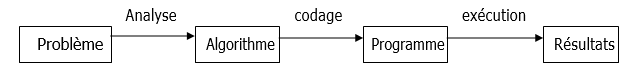
\includegraphics[scale=1]{img1.PNG} % insère une image en taille réelle
\end{figure}

L'ordinateur étant une machine totalement dénuée d'intelligence. Un programme exécute les instructions bien précises c'est-à-dire celle que le programmeur lui a donnée. Des erreurs ou des fantaisies lors de son exécution ne proviennent pas de l'ordinateur mais d'une erreur de conception.

\section{Paradigmes de programmation} % section 4

Un paradigme est un modèle ou "patron" de pensée, qui aide à définir un ensemble de règles ou de concepts permettant d'appréhender un cadre particulier. 
Ces concepts, adaptés à un domaine précis, permettent de voir un aspect de la réalité. 
Ainsi, chaque science dispose d'un ou plusieurs paradigmes adaptés à son sujet d'étude. 
En conséquence, la vision de chaque science sur un problème particulier est différente.

Les paradigmes en programmation désignent les principes fondamentaux du développement de logiciels. Au mieux, on peut se les représenter comme des styles de programmation fondamentaux divers générant des codes logiciels de structure différente.

\begin{figure}[h] % insère une figure ici (h = "here")
  \centering % centre la figure
  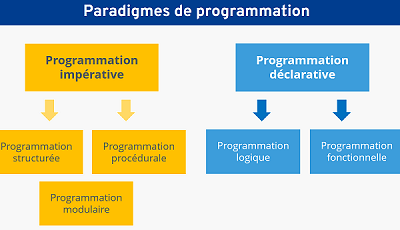
\includegraphics[scale=1]{paradigme.png} % insère une image en taille réelle
 
 Vue d’ensemble des principaux paradigmes de programmation
\end{figure}

Traditionnellement, la programmation impérative est la forme la plus courante. Son code source définit clairement la séquence d’étapes à exécuter par un programme. Il en existe plusieurs sous-catégories, parmi lesquelles la programmation procédurale et la programmation axée sur l’objet. Suivant le principe de la programmation déclarative, seul l’objectif du logiciel est décrit (soit uniquement le résultat, et non les différentes étapes). Il en existe plusieurs sous-catégories, parmi lesquelles la programmation fonctionnelle et la programmation logique. Comment distinguer ces paradigmes logiciels les uns des autres ?

\subsection{Programmation impérative : le paradigme de programmation traditionnel} % subsection1

Parmi les paradigmes de programmation, la programmation impérative est considérée comme « traditionnelle ». Les premiers langages de programmation et, de ce fait, les premiers programmes informatiques, ont été intégralement conçus sur cette base, qui énonce une séquence stricte d’ordres déterminés (du lat. imperare « ordonner ») ou, pour ainsi dire, des instructions d’exécution. Ce paradigme de programmation sert entre autres de base aux langages Pascal et C, ainsi qu’à tous les langages d’assemblage. En programmation impérative, l’accent est notamment mis sur une collaboration aussi étroite que possible avec le système. Le code de programmation en résultant est alors facile à comprendre, mais très volumineux.

Les programmations structurée, procédurale et modulaire sont trois approches majeures d’écriture et de structuration du code logiciel selon le paradigme programmation impérative.

\subsubsection{Programmation structurée}

L’approche de programmation structurée est une forme simplifiée de programmation impérative. La différence déterminante par rapport au principe de base : au lieu d’instructions de saut absolu (instructions entraînant le traitement, non pas avec l’ordre suivant, mais à un autre endroit), ce paradigme de programmation prévoit l’utilisation de boucles et structures de contrôle. Un exemple en est l’utilisation de « do...while » pour l’exécution automatique d’une instruction dès lors qu’une certaine condition est remplie (au moins une fois).

\subsubsection{Programmation procédurale}

Le paradigme de programmation procédurale étend l’approche impérative à la possibilité de subdiviser des algorithmes en plusieurs parties plus facilement maîtrisables. Celles-ci sont alors désignées par les termes procédures ou, selon le langage de programmation, sous-programmes, routines ou fonctions. L’objectif de cette subdivision est de faciliter la compréhension du code de programmation et d’éviter les répétitions de code inutiles.De par l’abstraction des algorithmes, le paradigme logiciel procédural s’impose comme une avancée déterminante entre les langages d’assemblage simples et les langages standard plus complexes.

\subsubsection{Programmation modulaire}

La programmation modulaire est également comprise comme une sous-catégorie du paradigme de programmation impérative. Elle est fondamentalement très similaire à l’approche procédurale et applique ce style de programmation aux exigences de projets logiciels plus volumineux et plus complets. Le code source est ici subdivisé de manière ciblée en blocs logiques indépendants les uns des autres pour plus de clarté et pour faciliter le processus de débogage (dépannage). Les différents blocs, encore appelés modules, peuvent être testés séparément avant d’être liés au sein d’une application commune.

\subsubsection{Quelques langages de programmation impérative les plus connus }: Fortran,Java,Pascal,ALGOL,C,C++,Assembler,BASIC,COBOL,Python,
Ruby...

\subsubsection{Avantages et inconvénients du paradigme de programmation impérative}

Avantage:
\begin{itemize}
   \item[$\bullet$]Bien lisible
   \item[$\bullet$]Comparativement facile à apprendre
   \item[$\bullet$]Modèle de pensée aisément compréhensible pour les débutants (étapes de résolution)
   \item[$\bullet$]Permet de tenir compte des caractéristiques de cas d’application spéciaux
\end{itemize}

Inconvenients:
\begin{itemize}
\item[$\bullet$]Le code devient très rapidement volumineux et perd en clarté
\item[$\bullet$]Risque d’erreurs supérieur lors de retouches
\item[$\bullet$]Les opérations de maintenance bloquent le développement d’applications, car la programmation est étroitement liée au système
\item[$\bullet$]Optimisations et extensions plus difficiles
\end{itemize}


\subsection{Programmation déclarative : paradigmes logiciels du passé récent} % subsection2

Parallèlement au développement continu de matériel et de logiciels, l’approche déclarative a permis l’élaboration d’un paradigme alternatif à la programmation de code. Le principe de base de la programmation déclarative réside ici dans la description du résultat final souhaité. Il s’agit donc en premier lieu de l’« objectif » à atteindre, et non du « déroulement » des étapes de résolution comme c’est le cas en programmation impérative. En programmation déclarative, le code est plus difficile à comprendre en raison de son haut niveau d’abstraction, mais est également plus court et plus précis.

Il existe des différences plus importantes entre les sous-catégories du paradigme de programmation déclarative qu’entre celles du style impératif. En outre, leur définition ou répartition n’est pas toujours très précise. Les deux approches principales du paradigme programmation déclarative sont la programmation fonctionnelle et la programme logique.


\subsubsection{Programmation fonctionnelle}

Tous les langages de programmation standard contiennent des fonctions. L’approche fonctionnelle du développement logiciel traite toutefois certaines fonctions de manière très particulière :

un programme fonctionnel se compose de fonctions ordonnées les unes par rapport aux autres, chaque partie de programme pouvant alors être conçue sous forme de fonction. Les fonctions peuvent prendre différents « statuts » au sein de la programmation fonctionnelle. Elles peuvent par exemple être liées les unes aux autres comme des données ou être utilisées sous forme de paramètres. Elles peuvent également être réutilisées sous forme de résultats fonctionnels. A contrario, le paradigme empêche l’affectation indépendante de valeurs.

D’une manière générale, cette sous-catégorie de programmation déclarative est très importante dans le domaine informatique et peut être utilisée de manière très variée. Le traitement spécial des fonctions permet aux programmateurs du domaine de définir et d’appliquer de nouvelles règles de calcul étendues à partir de fonctions.

\subsubsection{Programmation logique}

Le paradigme logiciel logique, également appelé programmation prédictive, repose sur la logique mathématique. Plutôt qu’une suite d’instructions, un logiciel programmé selon ce principe contient toute une gamme de principes, entendue comme une liste de faits et hypothèses. Chaque requête adressée au programme est traitée par un interpréteur. Celui-ci a recours à ces principes et applique des règles précédemment définies pour atteindre le résultat souhaité.

\subsubsection{Programmation orientée-objet}

Le paradigme orientée objets définit un ensemble d'objets qui interagissent entre eux. En d'autres termes : tout est objet. Elle n’améliore pas subitement la qualité de l’application comme par magie. En
revanche, elle aide à mieux organiser le code, à le préparer à des futures évolutions et à rendre certaines portions réutilisables pour gagner en temps et en clarté. C'est pour cela que les développeurs professionnels l'utilisent dans la plupart de leurs projets.
La POO se concentre dans la subdivision du problème sur les données.
\begin{itemize}
   \item[$\bullet$]La classe est la définition d’un type d’objets.
   \item[$\bullet$]L’encapsulation est le principe de cacher les détails d’implémentation de l’extérieur par une interface.
\end{itemize}

\subsubsection{Quelques langages de programmation déclarative les plus connus }
\begin{itemize}
   \item[$\bullet$]Prolog
   \item[$\bullet$]Java 
   \item[$\bullet$]C++
   \item[$\bullet$]Lisp
   \item[$\bullet$]ADA
   \item[$\bullet$]Haskell
   \item[$\bullet$]Miranda
   \item[$\bullet$]Erlang
   \item[$\bullet$]SQL...
\end{itemize}

\subsubsection{Avantages et inconvénients du paradigme de programmation déclarative}

Avantage:
\begin{itemize}
   \item[$\bullet$]Code plus court et plus efficace
   \item[$\bullet$]Exécutable par des méthodes encore inconnues au moment de la programmation
   \item[$\bullet$]Optimisation facile, grâce à la gestion de l’exécution par algorithme
   \item[$\bullet$]Maintenance possible indépendamment du développement de l’application
\end{itemize}

Inconvenients:
\begin{itemize}
\item[$\bullet$]Parfois difficile à comprendre par des tiers
\item[$\bullet$]Se fonde sur un modèle de pensée inhabituel pour l’homme (état de la solution)
\item[$\bullet$]Les caractéristiques de différents cas d’application ne peuvent que difficilement être prises en considération dans la programmation
\end{itemize}

\subsection{Comparaison entre les programmations impérative et déclarative}

Le paradigme de programmation impérative (paradigme axé sur les commandes) est le paradigme de base le plus ancien des deux. À l’inverse de la programmation déclarative, le développeur définit ici précisément, dans le code source, chacune des étapes à exécuter par l’ordinateur pour aboutir au résultat. Le « déroulement » prime. Cette approche se retrouve, par exemple, dans les langages de programmation Java, Pascal ou C. La programmation déclarative, au contraire, se concentre directement sur l’« objectif » à atteindre.

Voici un exemple d’application dans le domaine du montage de meubles : alors que la programmation impérative s’apparente à une notice de montage, la programmation déclarative donne pour modèle une image du meuble fini.

Plutôt que de laisser une marge d’exécution par l’utilisation de différentes fonctions, la programmation impérative utilise des variables qui sont transformées en durée d’exécution. Le code est plus long, mais aussi plus facile à comprendre que la forme abrégée et très abstraite du style déclaratif.

\section{Langages interprétés et langages compilés}

On peut distinguer deux grandes familles de langages : les langages interprétés et les langages compilés.

\subsection{Langages interprétés}
Le langage interprété est un langage de programmation dans lequel les instructions du programme sont traduit au fur et à mesure et exécutées aussitôt par un programme auxiliaire « l’interpréteur« , c’est celui-ci qui va exécuter le programme.
De ce fait l’exécution d’un programme interprété sera plus lente que celui d’un programme compilé.
Premièrement il lit l’instruction, deuxièmement il l’exécute et passe à l’instruction suivante
L’avantage du langage interprété est sa faciliter de programmation, il permet une exécution immédiate du programme même incomplet.

Voici une liste de quelques langages interprétés connus : – JavaScript, Perl, Python, BASIC,Prolog,Mathematica, etc.
\begin{figure}[h] % insère une figure ici (h = "here")
  \centering % centre la figure
  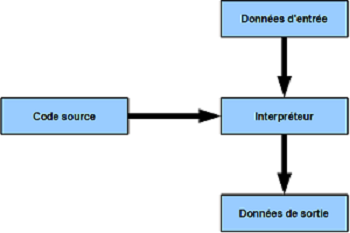
\includegraphics[scale=1]{interprete.png} % insère une image en taille réelle
\end{figure}

L'interprétation du code source est un processus « pas à pas » : l'interpréteur va exécuter les lignes du code une par une, en décidant à chaque étape ce qu'il va faire ensuite.

\subsection{Langages compilés}

Un langage compilé est un langage qui traduit toutes les instructions en une fois grâce à un programme auxiliaire, appelé compilateur, celui-ci va créer un fichier exécutable par le processeur et autonome.
Il a comme pour désavantages de devoir compiler le programme à chaque modification de celui-ci et que le programme est compilé pour un processeur donné, voire un système d’exploitation donné mais a pour avantages sa vitesse d’exécution, la phase de compilation permet d’identifier les erreurs de syntaxe et le programme compilé garantit la sécurité du code source ce qui est utile pour les applications sécurisées nécessitant la confidentialité du code (paiement en ligne, transaction bancaire, …).

Voici une liste de différents langages compilés : C, C++, CLEO, COBOL, etc.
\begin{figure}[h] % insère une figure ici (h = "here")
  \centering % centre la figure
  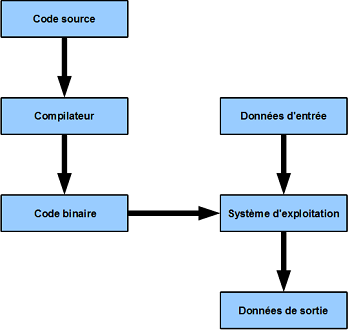
\includegraphics[scale=1]{compile.png} % insère une image en taille réelle
\end{figure}

\subsection{Principales différences}

On pourrait discuter très longtemps des avantages et inconvénients des différents types de langages mais les deux points qui sont les plus intéressants sont les suivants :

Dans un langage interprété, le même code source pourra marcher directement sur tout ordinateur. Avec un langage compilé, il faudra (en général) tout recompiler à chaque fois ce qui pose parfois des soucis.
Dans un langage compilé, le programme est directement exécuté sur l'ordinateur, donc il sera en général plus rapide que le même programme dans un langage interprété.

\section{Les autres types de langages de programmation}

\subsection{Langage de programmation événementielle}

La programmation événementielle permet le développement d'applications à interfaces graphiques.
Visual Basic, DLPHI, Visual C++, C++ builder, Visual J++, J++ builder, C sharp.

Un programme doit être écrit en langage d'évolué à l'aide d'un éditeur de texte. Le programme ainsi obtenu est appelé programmes sources ou code source.

Pour être utilisable, ce programme doit être traduit en langage machine. Le programme issu de cette traduction s'appelle programme objet.
La traduction du programme source en programme objet s'appelle la compilation et est réalisée par un programme spécialisé appelé compilateur.
La compilation permet de détecter les erreurs dues à un non-respect de la syntaxe du langage.

\subsection{Langages de scripts}

Les langages de script peuvent effectuer différentes actions dans un environnement d’exécution particulier, telles que l’automatisation de l’exécution de tâches, l’amélioration des fonctionnalités du logiciel parent, l’exécution de configurations, l’extraction de données à partir d’ensembles de données, et autres.
Quelques langage de Script: JavaScript,PHP,Python ,Ruby,Groovy,Perl,Lua,PowerShell,R,VBA,etc...

\subsection{Langage à balises}
Ces langages dits à balises servent à mettre en forme des documents électroniques pour être après utilisés en intranet, extranet ou pour la GEIDE (gestion de documents électroniques). Les données sont enregistrées entre des
« balises ». Il ne s'agit pas vraiment de langages, mais de format pour structurer les données qui pourront être exploitées à partir d'un simple navigateur.
\begin{itemize}
\item[$\bullet$]HTML (HyperText Markup Language)

HTML n'est pas vraiment un langages de programmation; c'est une technique pour coder des pages à l'aide de commandes de mise en forme. Ces dernières sont ensuite interprétées par le navigateur (browser en anglais) et sont affichés à l'écran.

\item[$\bullet$]XML

XML permet l'enregistrement, la gestion de la communication d'informations dans un format précis. Un document XML est utilisable à partir d'un simple navigateur récent.

\end{itemize}
\subsection{Langage de programmation Web}
\begin{itemize}
    \item[$\bullet$]PHP
    \item[$\bullet$]ASP
    \item[$\bullet$]Ruby
    \item[$\bullet$]Java Web
    \item[$\bullet$]Python,etc.
\end{itemize}

\section{Conclusion:Le choix}
Maintenant que nous avons vu dans les détail ce qu'est un langage de programmation, ses differents paradigmes; les types de langages de programmation, ainsi que les facilités que peuvent offrir les divers langages de programmation, et succinctement résumé ce que les langages existants fournissent, il convient de réaliser le but de cet article, c’est-à-dire choisir réellement un langage. 
Nous avions choisi de présenter trois situations typiques:
\begin{itemize}
    \item[$\bullet$]le débutant en programmation, qui cherche un premier langage ;
    \item[$\bullet$]l’amateur éclairé, qui veut réaliser un certain type de projet;
    \item[$\bullet$]l’ingénieur qui souhaite améliorer ses compétences. 
\end{itemize}

Pour chacune, le choix dependra de plusieurs critères à savoir: l'objectif du future logiciel à concevoir (Quels sont ses differentes fonctionalité);son future environement d'exécution;sa durée de conception, etc
Il n’y a pas de choix universellement reconnu comme « bon » néamoins, la puissance des langages tels que Python et Java, permet de nos jours grace à leurs technologies diverses de faciliter la conception de n'importe quel types d'application qu'elle soit Mobile, Web ou Destop. En revanche, il y a des choix ostensiblement médiocres.

\section{Références:}
\begin{itemize}
    \item[$\bullet$] [1] Histoire et évolution des langages de programmation Par Denis Sureau, 2014; 
    
    \item[$\bullet$] [2] Initiation à la programmation, M. Eleuldj, Département Génie Informatique, EMI, septembre 2014;
    
    \item[$\bullet$] [3] Gilles Dowek, Le langage mathématique et les langages de programmation, Colloque Voir, entendre, raisonner, calculer, Cité des sciences et de l'industrie, La Villette, Paris, 1997;
    
    \item[$\bullet$] [4] Comment choisir un langage de programmation, Thomas Pornin, Technique et Pratique, Collection dirigée par Emmanuel Cornet et Alexandre Hérault;
    
    \item[$\bullet$] [5] https://www.ionos.fr/digitalguide/;
    
    \item[$\bullet$] [6] http://www.france-ioi.org/;
    
    \item[$\bullet$] [7] https://fr.acervolima.com/;
    
    \item[$\bullet$] [8] Différence entre le langage compilé et interprété, écrit par SHUBHAMSINGH10 et traduit par Acervo Lima de Difference between Compiled and Interpreted Language. Licence: CCBY-SA;

    \item[$\bullet$] [9] Quelle est la différence entre langage interprété, semi-interprété et compilé ? Stephane Nachez , 12 mai 2018;
    
    \item[$\bullet$] [10] https://www.actuia.com/;
    \item[$\bullet$] [11] https://www.bocasay.com/fr/;
    \item[$\bullet$] [12] https://dept-info.labri.fr/;
    \item[$\bullet$] [13] Projet web : les questions à se poser pour bien choisir ses langages de développement , Par Mathieu le 30 juillet, 2020; 
    \item[$\bullet$] [14] Quel langage de programmation apprendre en 2021 ? ELODIE GOULAY ,18 FÉVRIER 2020;
    \item[$\bullet$] [15] Concept of Programing Languages, Robert W.Sebesta, 2006;
     \item[$\bullet$] [16] Quel langage de programmation choisir ? Publié par Elsa Moreira, 30 novembre 2021;
     \item[$\bullet$] [17] Paradigmes de programmation Une introduction Olivier PORTE CNRS Mai 2012; 
     \item[$\bullet$] [18] Les langages de programmation web les plus utilisés en 2020 ,Fév 06 2020, Daniel  
     \item[$\bullet$] [19] https://cherrypulp.com/fr/;
     \item[$\bullet$] [20] Programmation Procédurale VS POO 2022-01-02,Yan Morin
\end{itemize}
\end{document} % fin du corps du texte